%%%%%%
%
% $Author: Rakesh Patpalli$
% $Date: 26.05.2024 $
% $Path: BA24-02-Time-Series\report\Contents\en$
% $Version: 1.0 $
% $Reviewed by: Yogesh $
%
% !TeX encoding = utf8
% !TeX root = Rename
% !TeX TXS-program:bibliography = txs:///bibtex
%
%%%%%%

\chapter{Data Mining: XGBoost for Air Quality Forecasting}
\label{chapter 5}

\section{Introduction}

Significant progress has been made in artificial intelligence, especially in the field of machine learning. One of the most powerful and widely used algorithms in this field is XGBoost, which stands for Extreme Gradient Boosting. XGBoost is an implementation of gradient boosted decision trees designed for speed and performance. This chapter focuses on using XGBoost for time series forecasting of air quality data.

XGBoost has been selected as the primary model due to its superior performance in handling large datasets and its robustness in managing various types of data, including missing values and outliers. This makes XGBoost particularly suitable for predicting air quality parameters, which can be influenced by numerous environmental factors \cite{Chen:2016}.

XGBoost is an optimized distributed gradient boosting library designed for efficient and scalable training of machine learning models. It is an ensemble learning method that combines the predictions of multiple weak models to produce a stronger prediction \cite{Chen:2016}. One of the key features of XGBoost is its efficient handling of missing values, which allows it to handle real-world data with missing values without requiring significant pre-processing. Additionally, XGBoost has built-in support for parallel processing, making it possible to train models on large datasets in a reasonable amount of time \cite{Chen:2016}.

\section{Description}

XGBoost is an advanced machine learning algorithm based on decision tree ensembles. It is designed to be highly efficient, flexible, and portable. XGBoost implements a gradient boosting framework that can handle various data types and supports custom objective functions. It is known for its speed and performance, making it ideal for large-scale data mining tasks and real-time prediction scenarios \cite{Goodfellow:2016}.

The algorithm uses a second-order gradient to enhance the optimization process, providing better accuracy and convergence compared to first-order methods \cite{Chen:2016}. Regularization techniques are also incorporated to prevent overfitting, making the model more generalizable.

\section{Applications}

XGBoost is widely used across various domains due to its flexibility and high performance. Some of the key applications include:

\begin{itemize}
	\item \textbf{Time Series Forecasting:} Predicting future values in a time series, such as air quality indices, stock prices, and weather conditions \cite{Aggarwal:2015}.
	\item \textbf{Classification:} Identifying categories for given data points, such as spam detection, disease diagnosis, and image classification \cite{Goodfellow:2016}.
	\item \textbf{Regression:} Predicting continuous values, such as house prices, sales forecasts, and customer lifetime value \cite{Aggarwal:2015}.
	\item \textbf{Ranking:} Used in recommendation systems to rank products or content based on user preferences \cite{Chen:2016}.
\end{itemize}

\section{Relevance}

XGBoost is particularly relevant for the air quality forecasting project due to its ability to handle large datasets with high dimensionality and its robustness in managing missing values and outliers. It provides accurate and reliable predictions, which are essential for making informed decisions regarding air quality management and public health \cite{Chen:2016}.

\section{Hyperparameters}

Tuning hyperparameters in XGBoost is crucial for optimizing model performance. Some important hyperparameters include:

\begin{itemize}
	\item \textbf{Learning Rate:} Controls the step size during gradient descent. A smaller learning rate requires more boosting rounds \cite{Goodfellow:2016}.
	\item \textbf{Number of Estimators:} The number of trees in the ensemble. More trees can improve performance but increase computation time \cite{Chen:2016}.
	\item \textbf{Max Depth:} The maximum depth of each tree. Deeper trees can capture more information but may lead to overfitting \cite{Goodfellow:2016}.
	\item \textbf{Subsample:} The fraction of samples used for training each tree. Subsampling helps prevent overfitting \cite{Chen:2016}.
	\item \textbf{Colsample\_bytree:} The fraction of features used for training each tree. Reducing the number of features can also help prevent overfitting \cite{Aggarwal:2015}.
\end{itemize}

\section{Requirements}

To effectively use XGBoost for air quality forecasting, certain requirements must be met:

\begin{itemize}
	\item \textbf{Data Quality:} Ensure that the data is clean, with minimal missing values and outliers properly handled \cite{Chen:2016}.
	\item \textbf{Computational Resources:} Sufficient computational power to handle large datasets and perform intensive calculations \cite{Goodfellow:2016}.
	\item \textbf{Hyperparameter Tuning:} Adequate tools and techniques for hyperparameter optimization to enhance model performance \cite{Chen:2016}.
	\item \textbf{Real-time Processing:} Ability to process data and generate predictions in real-time for timely decision-making \cite{Aggarwal:2015}.
\end{itemize}

\section{Input}

Understanding the input data is crucial for building and training the XGBoost model. For the air quality forecasting project, the input data includes:

\begin{itemize}
	\item \textbf{Features:} PM2.5, PM10, NO2, SO2, CO, O3, temperature, humidity, wind speed, and other relevant parameters \cite{Chen:2016}.
	\item \textbf{Time Index:} A datetime index representing the timestamp of each observation \cite{Goodfellow:2016}.
	\item \textbf{Lag Features:} Generated to capture temporal dependencies by including past values of the target variable (e.g., PM2.5 levels from previous days) \cite{Chen:2016}.
\end{itemize}

\section{Output}

The output of the XGBoost model for air quality forecasting is a continuous value representing the predicted concentration of a specific air quality parameter (e.g., PM2.5) at a future time point. The model can generate predictions for various time horizons, such as the next hour, day, or week \cite{Goodfellow:2016}.

\section{Mathematics Behind XGBoost}

Before understanding XGBoost, it is essential to grasp the fundamentals of decision trees:

\subsection{Decision Tree}

A Decision tree is a flowchart-like tree structure, where each internal node denotes a test on an attribute, each branch represents an outcome of the test, and each leaf node (terminal node) holds a class label. A tree can be “learned” by splitting the source set into subsets based on an attribute value test. This process is repeated on each derived subset in a recursive manner called recursive partitioning. The recursion is completed when the subset at a node all has the same value of the target variable, or when splitting no longer adds value to the predictions \cite{Goodfellow:2016}.

\subsection{Bagging}

A Bagging classifier is an ensemble meta-estimator that fits base classifiers each on random subsets of the original dataset and then aggregate their individual predictions (either by voting or by averaging) to form a final prediction. Such a meta-estimator can typically be used as a way to reduce the variance of a black-box estimator (e.g., a decision tree), by introducing randomization into its construction procedure and then making an ensemble out of it. Each base classifier is trained in parallel with a training set which is generated by randomly drawing, with replacement, N examples from the original training dataset, where N is the size of the original training set. The training set for each of the base classifiers is independent of each other. Many of the original data may be repeated in the resulting training set while others may be left out \cite{Aggarwal:2015}.

\begin{figure}
	\centering
	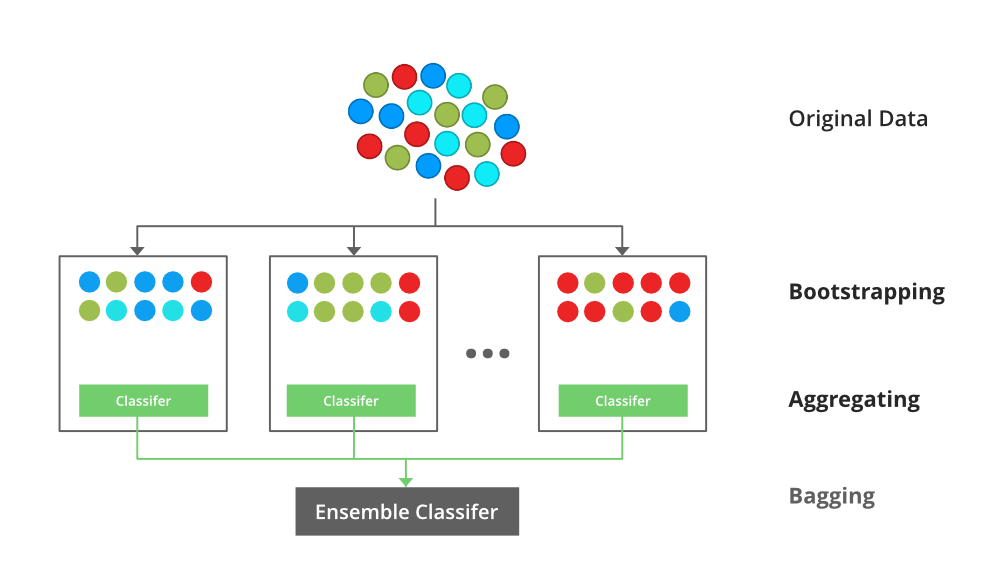
\includegraphics[width=0.8\textwidth]{Images/Bagging}
	\caption{Bagging Classifier} \label{fig:Bagging Classifier}
\end{figure}

\subsection{Random Forest}

Every decision tree has high variance, but when we combine all of them together in parallel then the resultant variance is low as each decision tree gets perfectly trained on that particular sample data and hence the output doesn’t depend on one decision tree but multiple decision trees. In the case of a classification problem, the final output is taken by using the majority voting classifier. In the case of a regression problem, the final output is the mean of all the outputs. This part is Aggregation. The basic idea behind this is to combine multiple decision trees in determining the final output rather than relying on individual decision trees. Random Forest has multiple decision trees as base learning models. We randomly perform row sampling and feature sampling from the dataset forming sample datasets for every model. This part is called Bootstrap \cite{Goodfellow:2016}.

\subsection{Boosting}

Boosting is an ensemble modelling technique that attempts to build a strong classifier from a number of weak classifiers. It is done by building a model using weak models in series. Firstly, a model is built from the training data. Then the second model is built which tries to correct the errors present in the first model. This procedure is continued and models are added until either the complete training data set is predicted correctly or the maximum number of models are added. Gradient Boosting is a popular boosting algorithm. In gradient boosting, each predictor corrects its predecessor’s error. In contrast to Adaboost, the weights of the training instances are not tweaked; instead, each predictor is trained using the residual errors of its predecessor as labels. There is a technique called the Gradient Boosted Trees whose base learner is CART (Classification and Regression Trees) \cite{Chen:2016}.

\begin{figure}
	\centering
	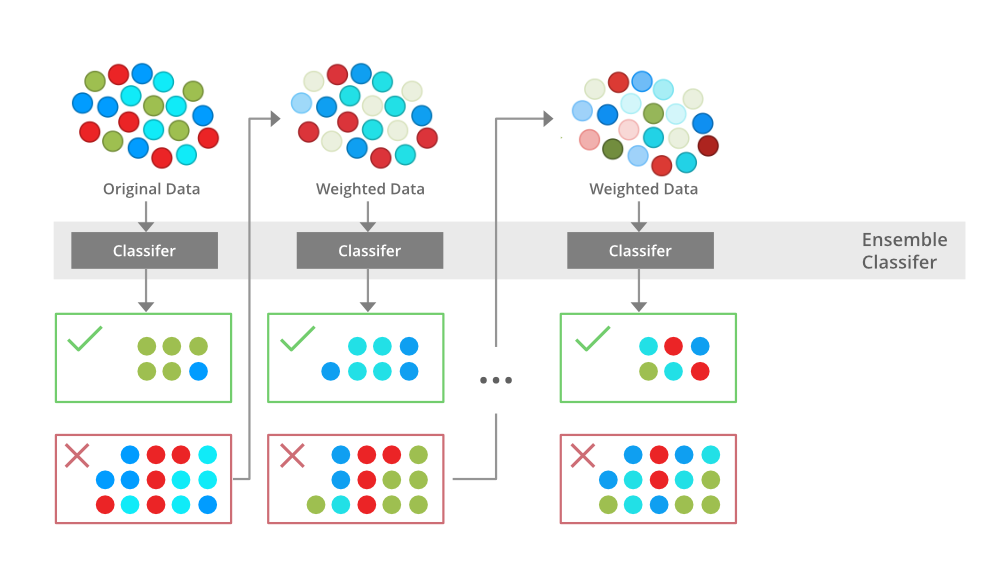
\includegraphics[width=0.8\textwidth]{Images/Boosting}
	\caption{Boosting Classifier} \label{fig:Boosting Classifier}
\end{figure}

\subsection{Mathematics behind XGBoost}

XGBoost is an implementation of Gradient Boosted decision trees. In this algorithm, decision trees are created in sequential form. Weights play an important role in XGBoost. Weights are assigned to all the independent variables which are then fed into the decision tree which predicts results. The weight of variables predicted wrong by the tree is increased and these variables are then fed to the second decision tree. These individual classifiers/predictors then ensemble to give a strong and more precise model. It can work on regression, classification, ranking, and user-defined prediction problems \cite{Chen:2016}.

Mathematically, we can write our model in the form:

\[
\hat{y}_{i} =  \sum_{k=1}^{K} f_k(x_i), f_k \epsilon \mathcal{F}
\]

where \(K\) is the number of trees, \(f\) is the functional space of \(F\), and \(F\) is the set of possible CARTs. The objective function for the above model is given by:

\[
\text{obj}(\theta) = \sum_{i}^{n} l(y_{i}, \hat{y}_{i}) + \sum_{k=1}^K \Omega(f_{k})
\]

where the first term is the loss function and the second is the regularization parameter. Instead of learning the tree all at once which makes the optimization harder, we apply the additive strategy, minimize the loss of what we have learned and add a new tree, which can be summarized below:

\[
\hat{y}_i^{(0)} = 0 \\
\hat{y}_i^{(1)} = f_1(x_i) = \hat{y}_i^{(0)} + f_1(x_i) \\
\hat{y}_i^{(2)} = f_1(x_i) + f_2(x_i) = \hat{y}_i^{(1)} + f_2(x_i) \\
... \\
\hat{y}_i^{(t)} = \sum_{k=1}^t f_k(x_i) = \hat{y}_i^{(t-1)} + f_t(x_i)
\]

The objective function of the above model can be defined as:

\[
\text{obj}^{(t)}  = \sum_{i=1}^{n} l(y_i, \hat{y}_{i}^{(t)}) + \sum_{i=1}^t\Omega(f_i) \\
= \sum_{i=1}^{n} l(y_i, \hat{y}_{i}^{(t-1)} + f_{t}(x_i)) + \Omega(f_t) + \text{constant}
\]

\[
\text{obj}^{(t)}  = \sum_{i=1}^n (y_{i} - (\hat{y}_{i}^{(t-1)} + f_t(x_i)))^2 + \sum_{i=1}^t\Omega(f_i) \\
= \sum_{i=1}^n [2(\hat{y}_i^{(t-1)} - y_i)f_t(x_i) + f_t(x_i)^2] + \Omega(f_t) + \text{constant}
\]

Now, let’s apply Taylor series expansion up to the second order:

\[
\text{obj}^{(t)} = \sum_{i=1}^{n} [l(y_i, \hat{y}_i^{(t-1)}) + g_i f_t(x_i) + \frac{1}{2} h_{i} f_{t}^2(x_i)] + \Omega(f_t) + \text{constant}
\]

where \(g_i\) and \(h_i\) can be defined as:

\[
g_i = \partial_{\hat{y}_i^{(t-1)}} l(y_i, \hat{y}_i^{(t-1)}) \\
h_i = \partial_{\hat{y}_i^{(t-1)}}^2 l(y_i, \hat{y}_i^{(t-1)})
\]

Simplifying and removing the constant:

\[
\sum_{i=1}^n [g_{i} f_{t}(x_i) + \frac{1}{2} h_{i} f_{t}^2(x_i)] + \Omega(f_t)
\]

Now, we define the regularization term, but first, we need to define the model:

\[
f_t(x) = w_{q(x)}, w \in R^{T}, q:R^d\rightarrow \{1,2,...,T\}
\]

Here, \(w\) is the vector of scores on leaves of the tree, \(q\) is the function assigning each data point to the corresponding leaf, and \(T\) is the number of leaves. The regularization term is then defined by:

\[
\Omega(f) = \gamma T + \frac{1}{2}\lambda \sum_{j=1}^T w_j^2
\]

Now, our objective function becomes:

\[
\text{obj}^{(t)} \approx \sum_{i=1}^n [g_i w_{q(x_i)} + \frac{1}{2} h_i w_{q(x_i)}^2] + \gamma T + \frac{1}{2}\lambda \sum_{j=1}^T w_j^2 \\
= \sum^T_{j=1} [(\sum_{i\in I_j} g_i) w_j + \frac{1}{2} (\sum_{i\in I_j} h_i + \lambda) w_j^2 ] + \gamma T
\]

Now, we simplify the above expression:

\[
\text{obj}^{(t)} = \sum^T_{j=1} [G_jw_j + \frac{1}{2} (H_j+\lambda) w_j^2] +\gamma T
\]

where,

\[
G_j = \sum_{i\in I_j} g_i \\
H_j = \sum_{i\in I_j} h_i
\]

In this equation, \(w_j\) are independent of each other, the best \(w_j\) for a given structure \(q(x)\) and the best objective reduction we can get is:

\[
w_j^{\ast} = -\frac{G_j}{H_j+\lambda} \\
\text{obj}^{\ast} = -\frac{1}{2} \sum_{j=1}^T \frac{G_j^2}{H_j+\lambda} + \gamma T
\]

where \(\gamma\) is the pruning parameter, i.e., the least information gain to perform a split.

Now, we try to measure how good the tree is. We can’t directly optimize the tree; we will try to optimize one level of the tree at a time. Specifically, we try to split a  leaf into two leaves, and the score it gains is:

\[
\text{Gain} = \frac{1}{2} \left[\frac{G_L^2}{H_L+\lambda}+\frac{G_R^2}{H_R+\lambda}-\frac{(G_L+G_R)^2}{H_L+H_R+\lambda}\right] - \gamma
\]

\section{Example with a Program}

The following Python code demonstrates how to use XGBoost for air quality forecasting:

\begin{lstlisting}[language=Python]
	import pandas as pd
	import numpy as np
	from xgboost import XGBRegressor
	from sklearn.model_selection import train_test_split, TimeSeriesSplit, RandomizedSearchCV, cross_val_score
	from sklearn.metrics import mean_squared_error, mean_absolute_error, r2_score
	import matplotlib.pyplot as plt
	import joblib
	
	# Load data
	df = pd.read_csv('air_quality_data.csv')
	df['From Date'] = pd.to_datetime(df['From Date'])
	df.set_index('From Date', inplace=True)
	
	# Feature Engineering
	def create_features(df):
	df['hour'] = df.index.hour
	df['day'] = df.index.day
	df['month'] = df.index.month
	df['year'] = df.index.year
	df['pm_lag_1Y'] = df['PM2.5 (ug/m3)'].shift(365*24)
	return df.dropna()
	
	df = create_features(df)
	
	# Split data into training and testing sets
	X = df.drop(['PM2.5 (ug/m3)'], axis=1)
	y = df['PM2.5 (ug/m3)']
	X_train, X_test, y_train, y_test = train_test_split(X, y, test_size=0.2, shuffle=False)
	
	# Train XGBoost model
	model = XGBRegressor(n_estimators=100, learning_rate=0.1, max_depth=5)
	model.fit(X_train, y_train)
	
	# Evaluate model
	predictions = model.predict(X_test)
	rmse = mean_squared_error(y_test, predictions, squared=False)
	mae = mean_absolute_error(y_test, predictions)
	r2 = r2_score(y_test, predictions)
	
	print(f"RMSE: {rmse}, MAE: {mae}, R2: {r2}")
	
	# Cross-validation
	tscv = TimeSeriesSplit(n_splits=5)
	scores = cross_val_score(model, X_train, y_train, cv=tscv, scoring='neg_mean_squared_error')
	print("Cross-validated scores:", scores)
	
	# Hyperparameter tuning
	param_distributions = {
		'n_estimators': [100, 150, 200],
		'learning_rate': [0.01, 0.05, 0.1],
		'max_depth': [3, 5, 7]
	}
	
	random_search = RandomizedSearchCV(model, param_distributions, n_iter=20, cv=tscv, scoring="neg_mean_squared_error")
	random_search.fit(X_train, y_train)
	best_model = random_search.best_estimator_
	
	# Feature importance
	importance = best_model.feature_importances_
	features = X_train.columns
	plt.barh(features, importance)
	plt.xlabel("Feature Importance")
	plt.ylabel("Feature")
	plt.title("Feature Importance from XGBoost")
	plt.show()
	
	# Future predictions
	def create_future_dataset(df, start_date, end_date):
	date_range = pd.date_range(start=start_date, end=end_date, freq='H')
	future_df = pd.DataFrame(index=date_range)
	future_df['hour'] = future_df.index.hour
	future_df['day'] = future_df.index.day
	future_df['month'] = future_df.index.month
	future_df['year'] = future_df.index.year
	for lag in [24, 48, 72, 96, 120, 144, 168, 336, 672]:
	future_df[f'pm_lag_{lag}H'] = df['PM2.5 (ug/m3)'].shift(lag)
	return future_df.dropna()
	
	future_df = create_future_dataset(df, start_date='2023-04-01', end_date='2024-03-30')
	future_predictions = best_model.predict(future_df)
	
	# Visualize future predictions
	plt.figure(figsize=(10, 5))
	plt.plot(future_df.index, future_predictions, label='Future Predictions')
	plt.xlabel('Date')
	plt.ylabel('PM2.5 (ug/m3)')
	plt.title('Future Air Quality Predictions')
	plt.legend()
	plt.show()
	
	# Save the best model
	joblib.dump(best_model, 'models/best_xgboost_model.pkl')
\end{lstlisting}

\section{Additional Considerations}

To further improve the performance and robustness of the XGBoost model, consider the following additional techniques and best practices:

\subsection{Ensemble Methods}

Combining multiple models can improve prediction accuracy. Techniques such as stacking, bagging, and boosting can be used to create a robust ensemble of models \cite{Goodfellow:2016}.

\begin{lstlisting}[language=Python]
	from sklearn.ensemble import StackingRegressor
	from sklearn.linear_model import Ridge
	
	# Define base models
	base_models = [('xgb', XGBRegressor()), ('ridge', Ridge())]
	
	# Define meta model
	meta_model = Ridge()
	
	# Create the stacking model
	stacking_model = StackingRegressor(estimators=base_models, final_estimator=meta_model)
	
	# Train the stacking model
	stacking_model.fit(X_train, y_train)
	
	# Evaluate the stacking model
	stacking_predictions = stacking_model.predict(X_test)
	stacking_rmse = mean_squared_error(y_test, stacking_predictions, squared=False)
	stacking_mae = mean_absolute_error(y_test, stacking_predictions)
	stacking_r2 = r2_score(y_test, stacking_predictions)
	
	print(f"Stacking RMSE: {stacking_rmse}, MAE: {stacking_mae}, R2: {stacking_r2}")
\end{lstlisting}

\subsection{Model Interpretation}

Understanding model predictions is crucial for trust and transparency. Use SHAP (SHapley Additive exPlanations) to interpret the output of your XGBoost model \cite{Goodfellow:2016}.

\begin{lstlisting}[language=Python]
	import shap
	
	# Create a SHAP explainer
	explainer = shap.Explainer(best_model, X_train)
	
	# Calculate SHAP values
	shap_values = explainer(X_test)
	
	# Plot SHAP values
	shap.summary_plot(shap_values, X_test)
\end{lstlisting}

\subsection{Handling Missing Data}

Ensure that missing data is handled appropriately. While XGBoost can handle missing values internally, it's often beneficial to understand and preprocess missing data before model training \cite{Chen:2016}.

\begin{lstlisting}[language=Python]
	# Fill missing values with median value of each column
	df.fillna(df.median(), inplace=True)
	
	# Alternatively, drop rows with missing values
	df.dropna(inplace=True)
\end{lstlisting}

\subsection{Data Augmentation}

Enhance your dataset by creating synthetic data points. This can help improve the model's ability to generalize \cite{Goodfellow:2016}.

\begin{lstlisting}[language=Python]
	from sklearn.utils import resample
	
	# Upsample minority class
	minority_class = df[df['PM2.5 (ug/m3)'] > df['PM2.5 (ug/m3)'].median()]
	upsampled_minority = resample(minority_class, replace=True, n_samples=len(df), random_state=42)
	
	# Combine majority class with upsampled minority class
	df_balanced = pd.concat([df, upsampled_minority])
	
	# Shuffle the dataset
	df_balanced = df_balanced.sample(frac=1).reset_index(drop=True)
\end{lstlisting}

\section{Conclusion}

This project demonstrated a comprehensive approach to analyzing and forecasting air quality data using the XGBoost model. The process involved detailed data preprocessing, feature engineering, exploratory analysis, and robust forecasting techniques. By leveraging advanced machine learning techniques, this project provides valuable insights for researchers, policymakers, and the general public, highlighting the potential of predictive modeling in addressing critical environmental challenges \cite{Goodfellow:2016}.

The use of XGBoost, with its efficiency and effectiveness in handling large datasets and various data types, proved to be a robust choice for this task \cite{Chen:2016}. Future work could involve integrating additional meteorological data, further hyperparameter tuning, and exploring other advanced ensemble methods to enhance predictive accuracy \cite{Aggarwal:2015}.